% Setup the document and basic packages
\documentclass[10pt,letterpaper,oneside]{book}
\usepackage{graphicx}
\usepackage{amsmath}
\usepackage{tabulary}
\usepackage{multirow}
\usepackage{ulem}
\usepackage{enumerate}
\usepackage{framed}
\usepackage{subfig}
\usepackage[pdftex,bookmarks=true]{hyperref}				
\hypersetup{colorlinks=true, linkcolor=blue, citecolor=blue, urlcolor=blue}

% Use the listing package for displaying code
\usepackage{listings}
\lstset{language=matlab,frame=top,frame=bottom, keywordstyle=\color{black}}

% Change the font to a sans serif font
\usepackage[T1]{fontenc}
\renewcommand*\familydefault{\sfdefault}

% Setup the page appearance
\usepackage[margin=1in, top=1in]{geometry}
\setlength\parindent{0pt}
\setlength{\parskip}{10pt}

% Define a few short-hand commands
\newcommand{\df}[2]{\ensuremath{\frac{d #1}{d #2}}}
\newcommand{\ddf}[2]{\ensuremath{\frac{d^2 #1}{d #2^2}}}
\newcommand{\pf}[2]{\ensuremath{\frac{\partial #1}{\partial #2}}}
\newcommand{\ppf}[2]{\ensuremath{\frac{\partial^2 #1}{\partial #2^2}}}
\newcommand{\e}[1]{\ensuremath{\times 10^{#1}}}	
\newcommand{\dgr}{\ensuremath{^{\circ}}}
\newcommand{\spr}[1]{\ensuremath{^{\textrm{#1}}}} 
\newcommand{\sub}[1]{\ensuremath{_{\textrm{#1}}}} 
\newcommand{\C}{\dgr C}
\newcommand{\F}{\dgr F}

% Define a command for the folder location (default is current directory)
\providecommand{\folder}{}

% Define a counter for keeping track of the assignment and question number
\newcounter{assignment}
\setcounter{assignment}{0}
\newcounter{question}
\setcounter{question}{0}

% Define a counter for only compiling a single question
\newcounter{outputnum}
\setcounter{outputnum}{0}
\newcommand{\buildonly}[1]{\setcounter{outputnum}{#1}}

% Change section apperance
\usepackage{titlesec}
\titleformat{\chapter}{}{}{0pt}{\Huge\textbf{Homework \arabic{assignment}}\\\huge}[\thispagestyle{empty}\normalsize]
\titleformat{\section}[hang]{}{}{0pt}{\Large\textbf}[\thispagestyle{empty}\normalsize]
\titleformat{\subsection}[hang]{}{}{0pt}{\large\textbf}[\thispagestyle{empty}\normalsize]

% Define a flag for showing solution and compiling a single question
\usepackage{xifthen}
\newboolean{solution}				% true - displays solutions
\newboolean{hidesolution} 			% true - hides solution and warning message (see \hidesolution command below)
\newboolean{header}					% true - displays the name and date header; false - the problem number

% Define a command for hiding the solution regardless of the status of solution flag, this is usefull if the solution is is build into the question
% as is the case with \tf command below. The command \hidesolution must be included inside every \question command that you want to hide
\newcommand\hidesolution{\setboolean{hidesolution}{true}}

% Define a command for a true/false question, includes the solution (use the \hidesolution command to supress warning message)
\providecommand\truefalse{True~|~False} % text to be printed

% \tf[solution]{This question is true...}, the solution is optional
\newcommand{\tf}[2][-NoValue-]{

	% Test if the solution flag is true
	\ifthenelse{\boolean{solution}}{ 
	
		% TRUE: the solution is desired
		\ifthenelse{\equal{#1}{-NoValue-}}{
			% We don't know the solution
			\renewcommand\truefalse{True~|~False}
		 }
		 {		
			% We know the solution
			\ifthenelse{\equal{#1}{T}}{ 
				% The solution is true
				\renewcommand\truefalse{\fbox{True}~|~\sout{False}}
			}{
				% The solution is false
				\renewcommand\truefalse{\sout{True}~|~\fbox{False}}
			}
		}		
	}
	{
		% FALSE: the solution was not wanted
		\renewcommand\truefalse{True~|~False}
	}
	
	\begin{tabulary}{\linewidth}{lL}
		\truefalse & #2 \\
	\end{tabulary}
	
}

% Define the question command
\newcommand\assignment[1]{

	% Reset question and equation counters
	\setcounter{equation}{0}
	\setcounter{question}{0}	
	
	% Increment assignment counter
	\addtocounter{assignment}{1}
	
	% Set the folder name
	\renewcommand{\folder}{#1}

	% Build the assigment
	\ifthenelse{\value{outputnum} = 0 \OR \value{outputnum} = \value{assignment}}{
		\pagestyle{empty}
		\input{#1/#1.tex}
	}{}
	
}

% Builds the question
\newcommand{\question}[1]{

	% Increment question counter
	\addtocounter{question}{1}

	% Insert the question
	\ifthenelse{\boolean{hidesolution}}{}{ 						% If hidesolution is true do nothing
		\ifthenelse{\boolean{solution}}{\newpage}{} 			% if false, insert a newpage
	} 					  
	\section{Problem \arabic{question}}
	The strong form of for the 1D heat conduction problem is given as follows, where $T$ is temperature, $k$ is thermal conductivity, $A$ is cross-sectional area, $s$ is the heat source, $q$ is heat flux. The domain is denoted as $\Omega$. The boundaries ares denoted as $\Gamma_T$ where the temperature is prescribed, $\Gamma_q$ where the flux is prescribed, and $\Gamma_h$ on the flux is known in terms of the convective heat transfer coefficient ($h$) and ambient temperature ($T_{\infty}$).

\begin{equation}\begin{split}\label{eq:strong}
& \df{}{x}\bigg({Ak \df{T}{x}}\bigg) + s = 0 \quad \text{on} \quad \Omega, \\
& \vec{q}\cdot \hat{n} = \bar{q} \quad \text{on} \quad \Gamma_q, \\
& \vec{q}\cdot \hat{n} = h(T - T_{\infty}) \quad \text{on} \quad \Gamma_h, \\
& T = \bar{T} \quad \text{on} \quad \Gamma_T.
\end{split}\end{equation}

Derive the weak form of Equation \eqref{eq:strong}, the finite element stiffness matrix, and the finite element force vector.
	
	% Insert the figure (if it exists)
	\IfFileExists{\folder /#1/fig.pdf}{
		\begin{center}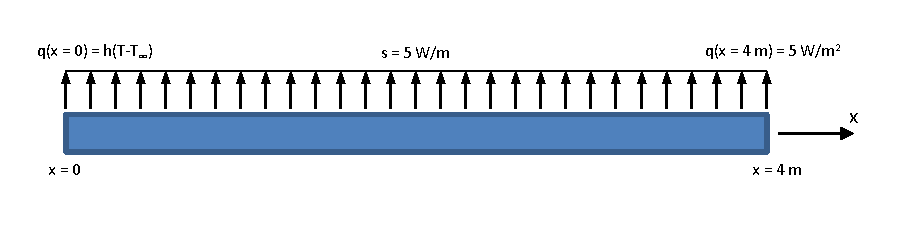
\includegraphics{\folder /#1/fig.pdf}\end{center}
	}{	
		\vspace{12pt}
	}
	
	% Insert the solution (if desired and if it exists)
	\ifthenelse{\boolean{hidesolution}}{}{ 						% If hidesolution is true do nothing
		\ifthenelse{\boolean{solution}}							% if false, insert the soln or a message if the soln.tex does not exist
		{
			\IfFileExists{\folder /#1/soln.tex}{
% 				\rule{\linewidth}{2pt}\vspace*{-10pt}
				\section*{Solution}
				Computing the temperature gradient involves looping over the elements, extracting the quadrature points and local values of the temperature solution, as shown in the following code. Which is applicable to both the Tutorial Problem and Problem 2.
\begin{lstlisting}
for e = 1:mesh.n_elements; % loop through the elements
    
    % Extract the current element from the mesh object
    elem = mesh.element(e);
    
    % Get the Gauss points
    qp = elem.quad.rules();
    
    % Collect the local values of T
    d(:,1) = T(elem.get_dof());
    
    % Compute the temperature gradient at the gauss point
    TG(e) = elem.shape_deriv(qp(1))*d;
    TGx(e) = elem.get_position(qp(1));   
end    
\end{lstlisting}
The temperature gradients for the tutorial are 72.5 \C/m and 22.5 \C/m for elements 1 and 2, respectively. For Problem 2 the gradients are 29.0 \C/m and -2.7\C/m.\par
% 				\rule{\linewidth}{2pt}\vspace*{-10pt}
			}{	
				\vspace{1em}
				
				\begin{center}
					\textbf{No solution exists for this question, to add solution create a file named:\\ ``\folder /\detokenize{#1}/soln.tex''}
				\end{center}
			}
		}{}
	}	
	% After every question the solution is allowed, the \nosolution command is needed inside every question that does not need a solution
	\setboolean{hidesolution}{false}
}
